% !TeX program = xelatex
\documentclass[12pt,a4paper]{ctexart}

% ============ 中文支持与字体 ============
\usepackage{ctex}
\setCJKmainfont{SimSun}[AutoFakeBold=3]
\setCJKsansfont{KaiTi}
\setCJKmonofont{SimHei}

% ============ 页面布局 ============
\usepackage[top=2.5cm, bottom=2.5cm, left=2.8cm, right=2.8cm]{geometry}

% ============ 颜色与图形 ============
\usepackage[dvipsnames,svgnames]{xcolor}
\usepackage{tikz}
\usetikzlibrary{shapes.geometric, arrows, positioning, fit, backgrounds, shadows, arrows.meta, calc, decorations.pathreplacing, automata}
\usepackage{tcolorbox}
\tcbuselibrary{skins, breakable}

% ============ 数学与算法 ============
\usepackage{amsmath, amssymb, amsthm}
\usepackage{mathtools}

% ============ 代码与列表 ============
\usepackage{listings}
\usepackage{enumitem}

% ============ 表格 ============
\usepackage{booktabs, tabularx, multirow}

% ============ 超链接与书签 ============
\usepackage{hyperref}
\hypersetup{
  colorlinks=true,
  linkcolor=NavyBlue,
  urlcolor=RoyalBlue,
  citecolor=ForestGreen,
  pdftitle={有限自动机 — Chapter 3-1 讲解},
  pdfauthor={Lecture Notes},
  pdfsubject={Finite Automata},
  pdflang={zh-CN},
  bookmarksnumbered=true,
  bookmarksopen=true
}

% ============ 自定义颜色 ============
\definecolor{mainblue}{HTML}{2B579A}
\definecolor{subblue}{HTML}{3A7BD5}
\definecolor{lightblue}{HTML}{E8F0FE}
\definecolor{accent}{HTML}{E74C3C}
\definecolor{codebg}{HTML}{F5F5F5}
\definecolor{notebg}{HTML}{FFF8E1}
\definecolor{warnbg}{HTML}{FFEBEE}

% ============ 自定义盒子样式 ============
\newtcolorbox{keybox}{
  colback=lightblue, colframe=mainblue, sharp corners, boxrule=0.5mm,
  fonttitle=\bfseries\sffamily, title=\textbf{核心概念}
}

\newtcolorbox{notebox}{
  colback=notebg, colframe=orange!60!yellow, sharp corners, boxrule=0.3mm,
  fonttitle=\bfseries, title=\textbf{📝 笔记}
}

\newtcolorbox{warnbox}{
  colback=warnbg, colframe=accent, sharp corners, boxrule=0.4mm,
  fonttitle=\bfseries, title=\textbf{⚠ 注意事项}
}

% ============ 自定义命令 ============
\newcommand{\term}[1]{\textbf{\textcolor{mainblue}{#1}}}
\newcommand{\enterm}[1]{\textbf{\textcolor{subblue}{#1}}}
\newcommand{\dfa}{\textit{DFA}\ }
\newcommand{\nfa}{\textit{NFA}\ }
\newcommand{\DFA}{\textit{DFA}\ }
\newcommand{\NFA}{\textit{NFA}\ }

% 章节标题样式
\usepackage{titlesec}
\titleformat{\section}
  {\normalfont\LARGE\bfseries\color{mainblue}}
  {\thesection}{1em}{}
\titleformat{\subsection}
  {\normalfont\Large\bfseries\color{subblue}}
  {\thesubsection}{1em}{}
\titleformat{\subsubsection}
  {\normalfont\large\bfseries}
  {\thesubsubsection}{1em}{}

% ============ 代码样式 ============
\lstset{
  basicstyle=\ttfamily\small,
  backgroundcolor=\color{codebg},
  frame=single,
  framerule=0.3mm,
  rulecolor=\color{gray!50},
  tabsize=2,
  breaklines=true,
  xleftmargin=1em,
  xrightmargin=1em
}

% ============ 文档信息 ============
\title{
  \vspace{2cm}
  {\Huge\bfseries\color{mainblue} 编译器导论}\\[0.5cm]
  {\Large\color{subblue} Chapter 3-1: Finite Automata}\\[0.3cm]
  {\Large 有限自动机}\\[1cm]
  {\normalsize\color{gray} 基于南京大学计算机学院课程讲义}\\[0.3cm]
  {\normalsize\color{gray} 时清凯 \texttt{|} qingkaishi@nju.edu.cn}
  \vspace{1cm}
}
\author{}
\date{\today}

\begin{document}

\maketitle
\thispagestyle{empty}

% ==================== 目录 ====================
\newpage
\setcounter{page}{1}
\tableofcontents
\newpage

% ==================== 前言 ====================
\section*{前言}
\addcontentsline{toc}{section}{前言}

本文是对《编译器导论》课程第三章第一部分 $\langle$Finite Automata$\rangle$ 的详细讲解笔记。原始讲义由南京大学计算机学院时清凯老师制作，共包含 124 页幻灯片。有限自动机是\emph{词法分析（Lexical Analysis）} 的理论基础，用于描述和识别\emph{正则语言（Regular Language）}。

本文按照原讲义的逻辑分为三个主要部分：

\begin{enumerate}[leftmargin=2em, itemsep=0.3em]
  \item \textbf{第一部分：数学预备知识} — 字母表、字符串、语言的操作与性质
  \item \textbf{第二部分：确定型有限自动机（DFA）} — DFA 的定义、语言识别、最小化、双向模拟等价性检验
  \item \textbf{第三部分：非确定型有限自动机（NFA）} — NFA 的定义、$\epsilon$-转移、NFA 到 DFA 的转换（子集构造法）
\end{enumerate}

\vspace{0.5cm}
有限自动机理论是编译原理中词法分析器的数学基础。理解 DFA 与 NFA 的关系，掌握 NFA $\rightarrow$ DFA 的转换方法，是实现词法分析器生成工具（如 lex/flex）的关键。

\newpage

% ==================== 第一部分：数学预备知识 ====================
\section{第一部分：数学预备知识（Math Preliminaries）}

在深入有限自动机之前，需要建立形式语言理论的基本概念。

\subsection{字母表与字符串（Alphabet and Strings）}

\begin{keybox}
  \term{语言（Language）} 是\emph{字符串的集合}，例如 $\{\, cat, dog, \dots \,\}$。

  \term{字符串（String）} 是定义在\emph{字母表（Alphabet）}上的\emph{字母（Letters）}序列。
\end{keybox}

\begin{itemize}[itemsep=0.2em]
  \item \textbf{字母表示例：} $\Sigma = \{a, b, c, d, \dots, z\}$
  \item \textbf{字符串示例：} cat, dog, apple, \dots
  \item \textbf{小型字母表示例：} $\Sigma = \{a, b\}$
  \begin{itemize}
    \item 在此字母表上可构成的字符串：$a$, $b$, $ab$, $aab$, $aabb$, $\dots$
    \item 语言是 $\{a, b, ab, aab, aabb, \dots\}$ 的任意子集
  \end{itemize}
\end{itemize}

\subsection{字符串操作（String Operations）}

\subsubsection{连接（Concatenation）}

两个字符串的连接是将它们头尾相接：

$$w_1 = aabb;\quad w_2 = bbaa \;\Longrightarrow\; w_1w_2 = aabbbbaa$$

\subsubsection{反转（Reverse）}

$$w = a_1a_2a_3a_4 \;\Longrightarrow\; w^R = a_4a_3a_2a_1$$

\subsubsection{长度（Length）}

字符串中字母的个数，记为 $|w|$：

$$w = a_1a_2a_3a_4 \;\Longrightarrow\; |w| = 4$$

\subsection{空字符串与子字符串}

\begin{keybox}
  \term{空字符串（Empty String）} 记为 $\epsilon$（epsilon），是长度为 0 的特殊字符串。
\end{keybox}

$$|\epsilon| = 0$$
$$\epsilon aabb = aab\epsilon\epsilon b = aabb\epsilon = aabb$$

\textbf{子字符串（Substring）：} 字符串中连续字符组成的子序列。例如 $abbab$ 的子串包括 $abbab$, $abba$, $bbab$, $abb$, $bba$, $\dots$

\textbf{前缀与后缀（Prefix and Suffix）：} 若 $w = uv$，则 $u$ 是前缀，$v$ 是后缀。
\begin{itemize}
  \item $abb$ 的前缀：$\epsilon$, $a$, $ab$, $abb$
  \item $abb$ 的后缀：$abb$, $bb$, $b$, $\epsilon$
\end{itemize}

\subsection{幂、Kleene 星号与加号}

\begin{keybox}
  \term{幂（Power）：} $w^n = \underbrace{ww\dots w}_{n\text{ 次}}$；特殊地，$w^0 = \epsilon$

  \term{Kleene 星号（Kleene Star）：} $\Sigma^*$ 表示由 $\Sigma$ 中字母构成的所有可能字符串的集合（包括 $\epsilon$）

  \term{加号（Plus）：} $\Sigma^+ = \Sigma^* - \{\epsilon\}$
\end{keybox}

\textbf{示例：}
\begin{itemize}[itemsep=0.2em]
  \item $(abb)^2 = abbabb$
  \item $(abb)^0 = \epsilon$
  \item $\Sigma = \{a, b\} \;\Longrightarrow\; \Sigma^* = \{\epsilon, a, b, ab, abb, aab, \dots\}$
  \item $\Sigma^+ = \{a, b, ab, abb, aab, \dots\}$
\end{itemize}

\begin{notebox}
  \textbf{重要结论：} 一个语言就是 $\Sigma^*$ 的任意子集。例如：$\{\epsilon\}$, $\{\epsilon, a, b\}$, $\emptyset$ 等等。

  \textbf{注意：} $\{\epsilon\} \neq \emptyset$！包含空字符串的集合不是空集。
\end{notebox}

\subsection{语言上的操作（Operations on Languages）}

\begin{keybox}
  语言本质上是\emph{集合}，因此集合操作自然适用于语言。此外，基于字符串操作可以定义语言特有的操作。
\end{keybox}

\subsubsection{集合操作}

令 $L_1 = \{a, b\}$，$L_2 = \{a, ab\}$：

\begin{itemize}[itemsep=0.2em]
  \item \textbf{并集：} $L_1 \cup L_2 = \{a, b, ab\}$
  \item \textbf{交集：} $L_1 \cap L_2 = \{a\}$
  \item \textbf{差集：} $L_1 - L_2 = \{b\}$
  \item \textbf{补集：} $\overline{L} = \Sigma^* - L$
  \item \textbf{反转：} $L^R = \{w^R : w \in L\}$
\end{itemize}

\subsubsection{连接、幂与闭包}

\begin{itemize}[itemsep=0.3em]
  \item \textbf{连接：} $L_1L_2 = \{xy : x \in L_1, y \in L_2\}$
  \item \textbf{幂：} $L^n = \underbrace{LL\dots L}_{n\text{ 次}}$；特殊地，$L^0 = \{\epsilon\}$
  \item \textbf{星闭包（Star-Closure）：} $L^* = L^0 \cup L^1 \cup L^2 \cup \cdots$
  \item \textbf{正闭包（Positive-Closure）：} $L^+ = L^1 \cup L^2 \cup \cdots = L^* - \{\epsilon\}$
\end{itemize}

\begin{notebox}
  \textbf{小测验：}
  \begin{enumerate}
    \item $L = \{a, b\}$，求 $L^2$ = ?
    \item $L = \{a^n b^n : n \geq 0\}$，求 $L^2$ = ?
  \end{enumerate}
  \textbf{答案：}
  \begin{enumerate}
    \item $L^2 = \{aa, ab, ba, bb\}$
    \item $L^2 = \{a^n b^n a^m b^m : n, m \geq 0\}$
  \end{enumerate}
\end{notebox}

\newpage

% ==================== 第二部分：确定性有限自动机 ====================
\section{第二部分：确定型有限自动机（DFA）}

\subsection{有限自动机的直观理解}

\begin{keybox}
  \term{有限自动机（Finite Automaton）} 是一种简单的计算模型：输入一个字符串，输出\emph{「接受（Accept）」}或\emph{「拒绝（Reject）」}。
\end{keybox}

\begin{figure}[ht]
\centering
\begin{tikzpicture}[
  node distance=2.5cm,
  box/.style={rectangle, draw=mainblue, thick, fill=lightblue, minimum size=1.2cm, align=center, rounded corners},
  arrow/.style={->, >=Stealth, thick}
]
  \node[box] (fa) {有限自动机\\Finite Automaton};
  \node[left=2cm of fa, align=center] (in) {字符串\\string};
  \node[right=2cm of fa, align=center] (out) {接受 accept\\或 拒绝 reject};
  \draw[arrow] (in) -- (fa);
  \draw[arrow] (fa) -- (out);
\end{tikzpicture}
\caption{有限自动机的输入输出模型}
\end{figure}

\textbf{以识别字符串 "abba" 的自动机为例：} 自动机从初始状态出发，每读入一个字符就按照转移规则跳转到下一个状态。读完所有字符后，若停在\emph{终止状态（Final State）}，则\emph{接受}该字符串；否则\emph{拒绝}。

例如输入 "abb"（而非 "abba"），读完后的状态不是终止状态，因此会被拒绝。

\subsection{DFA 的形式化定义}

\begin{keybox}
  一个\term{确定型有限自动机（DFA, Deterministic Finite Automaton）} 是一个五元组：
  $$M = (Q, \Sigma, \delta, q_0, F)$$
\end{keybox}

\textbf{五个组成部分：}
\begin{enumerate}[itemsep=0.3em]
  \item \enterm{$Q$：} 有限状态集合（A finite set of states）
  \item \enterm{$\Sigma$：} 有限输入字母表（A finite set of input characters / alphabet）
  \item \enterm{$\delta: Q \times \Sigma \mapsto Q$：} 转移函数（Transition function），如 $\delta(q, a) = q'$
  \item \enterm{$q_0 \in Q$：} 初始状态（The start state）
  \item \enterm{$F \subseteq Q$：} 终止状态集合（A finite subset of final states）
\end{enumerate}

\begin{notebox}
  \textbf{「确定型」的含义：} 对于任意状态 $q$ 和任意输入字符 $a$，转移函数 $\delta(q, a)$ 有\emph{且仅有唯一}的下一个状态。在任何时刻，自动机的行为是完全确定的。
\end{notebox}

\subsubsection{扩展转移函数}

\begin{keybox}
  \term{扩展转移函数 $\delta^*: Q \times \Sigma^* \mapsto Q$} 将单字符转移扩展为字符串转移：
  \begin{itemize}
    \item $\delta^*(q, abba) = q'$ （读完整个字符串后到达的状态）
    \item $\delta^*(q, \epsilon) = q$ （空字符串不改变状态）
  \end{itemize}
\end{keybox}

\subsection{DFA 定义的语言}

\begin{keybox}
  设 DFA $M = (Q, \Sigma, \delta, q_0, F)$，$M$ 所接受的语言定义为：
  $$L(M) = \{ w \in \Sigma^* : \delta^*(q_0, w) \in F \}$$
  即所有从初始状态出发、读完字符串后到达\emph{终止状态}的字符串集合。
\end{keybox}

\subsubsection{DFA 的实现：字符串检查器}

\begin{lstlisting}[language=C, caption={使用 DFA 检查字符串是否属于语言}]
void check(w, M) {
  q = q0;
  while (true) {
    c = read(w);
    if (c == None) {
      print(q in F ? "accept" : "reject");
      return;
    }
    switch (q) {
      case q0: if (c == 'a') { q = q1; } break;
      case q1: ... break;
      case q2: print("accept"); return;  // q2 in F
      case ...
    }
  }
}
\end{lstlisting}

\subsection{DFA 最小化（DFA Minimization）}

\begin{keybox}
  \term{DFA 最小化} 的目标是减少 DFA 的状态数，从而提高计算效率。等价的 DFA 可以有不同的状态数，最小化可以找到状态数最少的等价 DFA。
\end{keybox}

\subsubsection{最小化算法}

\textbf{核心思想：} 反复将状态划分为\emph{等价类（Equivalence Classes）}，使得同一等价类中的状态在任意输入下行为一致。

\textbf{算法步骤（以 6 状态 DFA 为例）：}

\begin{figure}[ht]
\centering
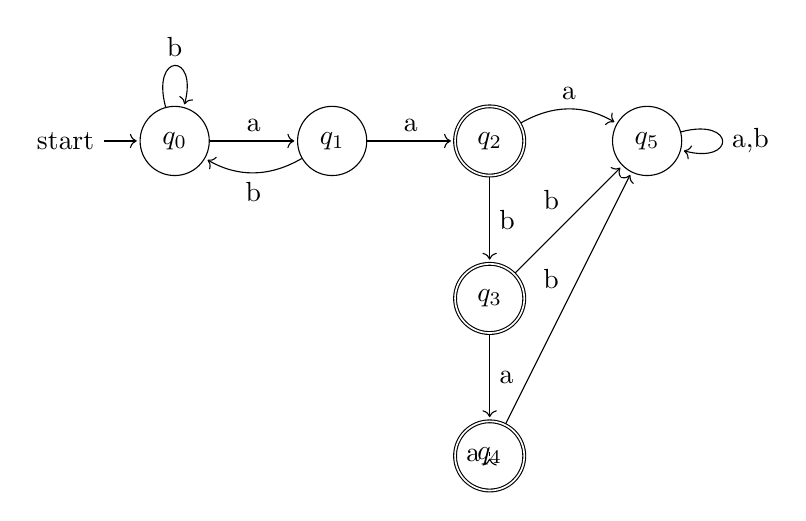
\begin{tikzpicture}[shorten >=1pt, node distance=2cm, on grid, auto]
  \node[state, initial] (q0) {$q_0$};
  \node[state] (q1) [right=of q0] {$q_1$};
  \node[state, accepting] (q2) [right=of q1] {$q_2$};
  \node[state, accepting] (q3) [below=of q2] {$q_3$};
  \node[state, accepting] (q4) [below=of q3] {$q_4$};
  \node[state] (q5) [right=of q2] {$q_5$};

  \path[->]
    (q0) edge node {a} (q1)
    (q0) edge [loop above] node {b} ()
    (q1) edge node {a} (q2)
    (q1) edge [bend left] node {b} (q0)
    (q2) edge [bend left] node {a} (q5)
    (q2) edge node {b} (q3)
    (q3) edge node {a} (q4)
    (q3) edge node {b} (q5)
    (q4) edge [bend left] node {a} (q4)
    (q4) edge node {b} (q5)
    (q5) edge [loop right] node {a,b} ();
\end{tikzpicture}
\caption{一个 6 状态的 DFA（最小化前）}
\end{figure}

\vspace{0.5em}
\begin{table}[h]
\centering
\begin{tabular}{@{}c|l|l@{}}
\toprule
\textbf{步骤} & \textbf{划分结果} & \textbf{说明} \\
\midrule
Step 1 & $\{q_0, q_1, q_5\}, \{q_2, q_3, q_4\}$ & 区分终止状态和非终止状态 \\
Step 2 & $\{q_0, q_1\}, \{q_5\}, \{q_2, q_3, q_4\}$ &
  $\delta(q_0, a/b)$ 和 $\delta(q_1, a/b)$ 在同一集合\\
  & & 但 $\delta(q_5, a/b)$ 不在 \\
Step 3 & $\{q_0, q_1\}, \{q_5\}, \{q_2, q_3, q_4\}$ & 结果不再变化，算法终止 \\
\bottomrule
\end{tabular}
\caption{DFA 最小化的划分过程}
\end{table}

\subsubsection{最小化结果}

最小化后，等价的原始 DFA 变为只有 \textbf{3 个状态}的 DFA：$q_{0,1}$（合并 $q_0, q_1$），$q_{2\sim4}$（合并 $q_2, q_3, q_4$），$q_5$。

\begin{notebox}
  \textbf{注意事项：}
  \begin{itemize}
    \item 在执行上述划分步骤之前，需要先\emph{移除所有不可达状态（Unreachable States）}
    \item DFA 最小化的最优平均时间复杂度为 $O(n \log\log n)$（Hopcroft 算法）
  \end{itemize}
\end{notebox}

\subsection{DFA 双向模拟（DFA Bi-Simulation）}

\begin{keybox}
  \term{DFA 双向模拟（Bi-Simulation）} 用于检查两个 DFA 的\emph{等价性}，即验证 $L(M_1) = L(M_2)$。
\end{keybox}

\textbf{基本原理：} 对于任意输入字符串，$M_1$ 到达终止状态\emph{当且仅当} $M_2$ 到达终止状态。

\textbf{方法：构造状态对表}，同时跟踪两个 DFA 在相同输入下的行为：

\begin{figure}[ht]
\centering
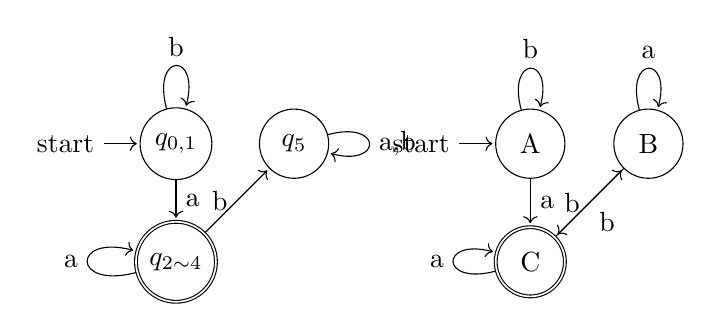
\begin{tikzpicture}[shorten >=1pt, node distance=2cm, on grid, auto]
  % DFA M1 (minimized)
  \node[state, initial] (q01) {$q_{0,1}$};
  \node[state] (q5) [right=1.5cm of q01] {$q_5$};
  \node[state, accepting] (q24) [below=1.5cm of q01] {$q_{2\sim4}$};

  \path[->]
    (q01) edge node {a} (q24)
    (q01) edge [loop above] node {b} ()
    (q24) edge [loop left] node {a} ()
    (q24) edge node [left] {b} (q5)
    (q5) edge [loop right] node {a,b} ();

  % DFA M2
  \node[state, initial] (A) [right=3cm of q5] {A};
  \node[state] (B) [right=1.5cm of A] {B};
  \node[state, accepting] (C) [below=1.5cm of A] {C};

  \path[->]
    (A) edge node {a} (C)
    (A) edge [loop above] node {b} ()
    (B) edge [loop above] node {a} ()
    (B) edge node {b} (C)
    (C) edge node [left] {b} (B)
    (C) edge [loop left] node {a} ();
\end{tikzpicture}
\caption{两个待比较的 DFA}
\end{figure}

通过构造状态对 $(q_i, s_j)$，跟踪两个 DFA 在每种输入下的共同行为。若对于所有可达的状态对，$M_1$ 的状态在 $F_1$ 中当且仅当 $M_2$ 的状态在 $F_2$ 中，则两个 DFA 等价。

\newpage

% ==================== 第三部分：非确定型有限自动机 ====================
\section{第三部分：非确定型有限自动机（NFA）}

\subsection{NFA 的直观理解}

\begin{keybox}
  \term{非确定型有限自动机（NFA, Non-deterministic Finite Automaton）} 在每个状态下对于同一个输入字符，可能存在\emph{多个可选的状态转移}。
\end{keybox}

\textbf{非确定性的含义：}
\begin{itemize}[itemsep=0.2em]
  \item 对于输入字符串 $aa$，第一条字符 $a$ 就可能有\emph{两种转移选择}
  \item 如果某条路径无法接受字符串，需要\emph{回溯尝试其他路径}
  \item 只要\emph{存在一条计算路径}能够接受字符串，该字符串就被 NFA 接受
\end{itemize}

\subsection{$\epsilon$ 转移（$\epsilon$-Transition）}

\begin{keybox}
  \term{$\epsilon$-转移} 允许 NFA 在不消耗任何输入字符的情况下\emph{自发地}转移到下一个状态。
\end{keybox}

这是 DFA 与 NFA 的一个重要区别——NFA 的转移函数接受 $\epsilon$ 作为输入。

\subsection{NFA 的形式化定义}

\begin{keybox}
  一个\term{非确定型有限自动机（NFA）} 是一个五元组：
  $$M = (Q, \Sigma \cup \{\epsilon\}, \delta, q_0, F)$$

  与 DFA 的关键区别在于转移函数：
  \begin{itemize}
    \item \textbf{DFA:} $\delta: Q \times \Sigma \mapsto Q$（确定性，唯一目标状态）
    \item \textbf{NFA:} $\delta: Q \times (\Sigma \cup \{\epsilon\}) \mapsto 2^Q$（非确定性，目标状态集合）
  \end{itemize}
\end{keybox}

\subsection{$\epsilon$-闭包（$\epsilon$-Closure）}

\begin{keybox}
  \term{$\epsilon$-closure($q$)} 返回从状态 $q$ 出发，通过零个或多个 $\epsilon$-转移能到达的所有状态集合，\emph{包括 $q$ 本身}。
\end{keybox}

\textbf{扩展转移函数 $\delta^*: Q \times \Sigma^* \mapsto 2^Q$：}

$q' \in \delta^*(q, w)$（其中 $w \in \Sigma^*$）当且仅当：
\begin{enumerate}
  \item 存在一条从 $q$ 到 $q''$ 的路径消耗了字符串 $w$
  \item 且 $q' \in \text{$\epsilon$-closure}(q'')$
\end{enumerate}

\subsection{NFA 定义的语言}

\begin{keybox}
  回顾 DFA 定义的语言：
  $$L(M) = \{ w \in \Sigma^* : \delta^*(q_0, w) \in F \}$$

  NFA 定义的语言类似，但条件是到达的状态集合与 $F$ 的\emph{交集非空}：
  $$L(M) = \{ w \in \Sigma^* : \delta^*(q_0, w) \cap F \neq \emptyset \}$$
  即\emph{存在至少一条路径}能够到达某个终止状态。
\end{keybox}

\subsection{NFA = DFA：两个模型的等价性}

\begin{keybox}
  \term{NFA 与 DFA 的表达能力是等价的}：
  \begin{itemize}
    \item 每个 DFA 天然就是一个 NFA（平凡情况）
    \item 每个 NFA 都可以转换为等价的 DFA（子集构造法）
    \item 即对于任意 NFA $N$，都存在 DFA $D$，使得 $L(N) = L(D)$
  \end{itemize}
\end{keybox}

\subsection{NFA 到 DFA 的转换：子集构造法}

\begin{keybox}
  \textbf{核心思想：} DFA 的每个状态对应于 NFA 的一个\emph{状态集合（子集）}。通过模拟 NFA 在每种输入下可能到达的所有状态集合来构建 DFA。
\end{keybox}

\textbf{算法步骤：}

\begin{enumerate}[itemsep=0.3em]
  \item \textbf{Step 1：} 初始化 DFA，起始状态为 $\{q_0\}$（NFA 初始状态的单元素集合）
  \item \textbf{Step 2：} 对于 DFA 的每个状态 $\{q_i, q_j, \dots, q_k\}$ 和每个字母 $a \in \Sigma$，计算：
  $$S = \bigcup_{q \in \{q_i, q_j, \dots, q_k\}} \delta^*(q, a)$$
  \item \textbf{Step 3：} 在 DFA 中添加转移：
  $$\delta_{\text{DFA}}(\{q_i, q_j, \dots, q_k\}, a) = S$$
  若 $S$ 中有任何状态是 NFA 的终止状态，则 $S$ 是 DFA 的终止状态
\end{enumerate}

\subsubsection{转换示例}

给定一个 NFA：

\begin{figure}[ht]
\centering
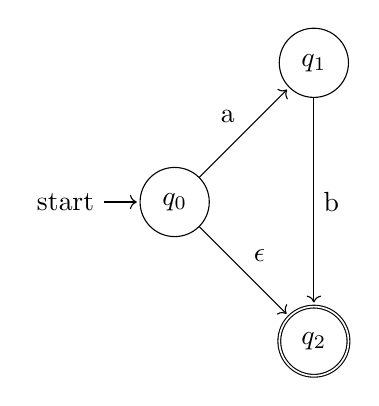
\begin{tikzpicture}[shorten >=1pt, node distance=2.5cm, on grid, auto]
  \node[state, initial] (q0) {$q_0$};
  \node[state] (q1) [above right=of q0] {$q_1$};
  \node[state, accepting] (q2) [below right=of q0] {$q_2$};

  \path[->]
    (q0) edge node {a} (q1)
    (q0) edge node {$\epsilon$} (q2)
    (q1) edge node {b} (q2);
\end{tikzpicture}
\caption{NFA 示例：识别 a 或 ab}
\end{figure}

\textbf{转换过程：}
\begin{itemize}[itemsep=0.2em]
  \item 初始 DFA 状态：$\{q_0\}$
  \item $\delta(\{q_0\}, a) = \{q_1, q_2\}$（新建 DFA 状态）
  \item $\delta(\{q_1, q_2\}, a) = \emptyset$
  \item $\delta(\{q_1, q_2\}, b) = \{q_2\}$（$\{q_2\}$ 包含终止状态 $\Rightarrow$ 是 DFA 终止状态）
\end{itemize}

\begin{warnbox}
  \textbf{NFA 转 DFA 的状态爆炸（State Explosion）：}

  因为 DFA 的状态是 NFA 状态的子集，一个 $n$ 状态的 NFA 在最坏情况下可能转换为最多 $2^n$ 状态的 DFA。对于每个 $n$，存在 $n$ 状态的 NFA 使得其所有子集都可达，因此转换后的 DFA 恰好有 $2^n$ 个状态，最坏时间复杂度为 $\Theta(2^n)$。

  \textbf{重要：} 将 NFA 转换为 DFA 时，不保证会得到规模更小的 DFA！
\end{warnbox}

\newpage

% ==================== 总结 ====================
\section{课程总结}

本章作为词法分析的理论基础，涵盖了以下核心要点：

\begin{enumerate}[itemsep=0.3em]
  \item \textbf{形式语言基础：} 字母表 $\Sigma$、字符串、语言（$\Sigma^*$ 的子集）、字符串与语言上的各种操作（连接、幂、Kleene 星号、正闭包等）

  \item \textbf{确定型有限自动机（DFA）：}
  \begin{itemize}
    \item 五元组定义：$(Q, \Sigma, \delta, q_0, F)$
    \item 语言定义：$L(M) = \{w \in \Sigma^* : \delta^*(q_0, w) \in F\}$
    \item \textbf{DFA 最小化：} 通过状态划分（初始划分终止/非终止状态，反复细化）减少状态数
    \item \textbf{DFA 双向模拟：} 通过跟踪状态对来检验两个 DFA 是否接受相同的语言
  \end{itemize}

  \item \textbf{非确定型有限自动机（NFA）：}
  \begin{itemize}
    \item 允许\emph{多条转移路径}和\emph{$\epsilon$-转移}
    \item 语言定义：$L(M) = \{w \in \Sigma^* : \delta^*(q_0, w) \cap F \neq \emptyset\}$
    \item \textbf{NFA = DFA：} 表达能力等价
    \item \textbf{子集构造法：} 将 NFA 转换为 DFA，最坏情况下产生指数级状态增长 $\Theta(2^n)$
  \end{itemize}

  \item \textbf{在编译器中的地位：}
  \begin{itemize}
    \item DFA/NFA 定义的语言 = 正则语言（Regular Language）
    \item 正则语言 $\leftrightarrow$ 正则表达式 $\leftrightarrow$ 有限自动机
    \item 词法分析器（Lexer）正是基于此理论构造的
  \end{itemize}
\end{enumerate}

\vfill
\begin{center}
\rule{0.5\textwidth}{0.3mm}\\[0.5em]
{\large\bfseries\color{mainblue} 本文完}\\[0.3em]
{\small 下一章将介绍正则表达式以及如何从正则表达式构建词法分析器。}
\end{center}

\end{document}
